\documentclass{article}
\usepackage{graphicx}
\graphicspath{ {./report_img/} } % graphics path
\usepackage{fancyhdr}
\usepackage{listings}
\setlength{\parindent}{0pt}
\usepackage{float}
\usepackage[letterpaper,margin=1in]{geometry}
\renewcommand{\baselinestretch}{1.2}    % line spacing
\usepackage{amsmath}
\usepackage{amssymb} % for \mathbb -- set of integers
%\usepackage[bf,large]{caption}
\usepackage{caption}
\usepackage{subcaption} % for subfigure environment
\usepackage{steinmetz}  % for \phase
\usepackage{mathrsfs}   % for \mathscr -- Laplace transform operator
\usepackage{mathtools}  % for \floor{}
\usepackage{sectsty}
\usepackage[usenames,dvipsnames]{color}
\definecolor{lightgray}{gray}{0.5}
% This is the color used for MATLAB comments below
\definecolor{MyDarkGreen}{rgb}{0.0,0.4,0.0}
\lstloadlanguages{Matlab}%
\lstset{language=bash,                        % Use MATLAB
        frame=single,                           % Single frame around code
        basicstyle=\small\ttfamily,             % Use small true type font
        %keywordstyle=[1]\color{Blue}\bf,        % MATLAB functions bold and blue
        %keywordstyle=[2]\color{Purple},         % MATLAB function arguments purple
        %keywordstyle=[3]\color{Blue}\underbar,  % User functions underlined and blue
        identifierstyle=,                       % Nothing special about identifiers
                                                % Comments small dark green courier
        commentstyle=\usefont{T1}{pcr}{m}{sl}\color{MyDarkGreen}\small,
        stringstyle=\color{Purple},             % Strings are purple
        showstringspaces=false,                 % Don't put marks in string spaces
        tabsize=2,                              % 5 spaces per tab
        %
        morecomment=[l][\color{Blue}]{...},     % Line continuation (...) like blue comment
        numbers=left,                           % Line numbers on left
        firstnumber=0,                          % Line numbers start with line 1
        numberstyle=\tiny\color{Blue},          % Line numbers are blue
        stepnumber=1,                           % Line numbers go in steps of 5
        breaklines=true
        }
\pagestyle{fancy}
%\thispagestyle{plain}

\def\class{ECE 408}
\def\fp{Final Project}

\partfont{\centering}

\lhead{ Sun, Xue, Miao, \class, \fp}

\begin{document}

\title{\fp}
\date{} % disable date to include in the title
\author{
\begin{tabular}{ccc}
    Alvin Sun & Yuqi Xue & Yan Miao \tabularnewline
    yixiaos3 & yuqixue2 & yanmiao2
\end{tabular}
}
%\maketitle

\begin{titlepage} % Suppresses displaying the page number on the title page and the subsequent page counts as page 1
	\newcommand{\HRule}{\rule{\linewidth}{0.5mm}} % Defines a new command for horizontal lines, change thickness here

	\center % Centre everything on the page

	%------------------------------------------------
	%	Headings
	%------------------------------------------------

	\textsc{\LARGE University of Illinois at Urbana Champaign}\\[1.5cm] % Main heading such as the name of your university/college

	\textsc{\Large Applied Parallel Programming}\\[0.5cm] % Major heading such as course name

	\large Team: wandering-gpu \\[0.5cm] % Minor heading such as course title

	%------------------------------------------------
	%	Title
	%------------------------------------------------

	\HRule\\[0.4cm]

	{\huge\bfseries Final Project}\\[0.4cm] % Title of your document

	\HRule\\[1.5cm]

	%------------------------------------------------
	%	Author(s)
	%------------------------------------------------

	\begin{minipage}{0.4\textwidth}
		\begin{flushleft}
			\large
			\textit{Author}\\
			Alvin Sun \\ % Your name
            Yuqi Xue  \\
            Yan Miao
		\end{flushleft}
	\end{minipage}
	~
	\begin{minipage}{0.4\textwidth}
		\begin{flushright}
			\large
			\textit{Net ID}\\
			yixiaos3 \\ % net id
            yuqixue2 \\
            yanmiao2
		\end{flushright}
	\end{minipage}

	% If you don't want a supervisor, uncomment the two lines below and comment the code above
	%{\large\textit{Author}}\\
	%John \textsc{Smith} % Your name

	%------------------------------------------------
	%	Date
	%------------------------------------------------

	\vfill\vfill\vfill % Position the date 3/4 down the remaining page

	{\large\today} % Date, change the \today to a set date if you want to be precise

	%------------------------------------------------
	%	Logo
	%------------------------------------------------

	%\vfill\vfill
	%\includegraphics[width=0.2\textwidth]{placeholder.jpg}\\[1cm] % Include a department/university logo - this will require the graphicx package

	%----------------------------------------------------------------------------------------

	\vfill % Push the date up 1/4 of the remaining page

\end{titlepage}

% deprecated
% \part*{Credentials}
% \setcounter{section}{0}
%
% \begin{tabular}{ll}
%     \textbf{Team Name}: & wandering-gpu \tabularnewline
%     \textbf{School Affiliation}: & UIUC \tabularnewline
%     \tabularnewline
% \end{tabular} \\
% \begin{tabular}{ll}
%     \textbf{Name}: & Alvin Sun \tabularnewline
%     \textbf{NetID}: & yixiaos3 \tabularnewline
%     \textbf{RaiID}: & 5c78c49784318364bab96ed4 \tabularnewline
%     \tabularnewline
%     \textbf{Name}: & Yuqi Xue \tabularnewline
%     \textbf{NetID}: & yuqixue2 \tabularnewline
%     \textbf{RaiID}: & 5c78c49f84318364bab96ee2 \tabularnewline
%     \tabularnewline
%     \textbf{Name}: & Yan Miao \tabularnewline
%     \textbf{NetID}: & yanmiao2 \tabularnewline
%     \textbf{RaiID}: & 5c78c48d84318364bab96ec2
% \end{tabular}

\part*{Milestone 1}
\setcounter{section}{0}

\section{Kernel Statistics}
\begin{tabular}{ccccccl}
 Time(\%) & Time & Calls & Avg & Min &   Max  &  Name \tabularnewline
  40.10\% &  16.788ms &  20 & 839.42us & 1.1200us & 16.155ms & [CUDA memcpy HtoD] \tabularnewline
  20.18\% & 8.4497ms  &  1 &  8.4497ms & 8.4497ms & 8.4497ms & void cudnn::detail::implicit\_convolve\_sgemm \tabularnewline
  11.81\% & 4.9434ms  &  1 &  4.9434ms & 4.9434ms & 4.9434ms & volta\_cgemm\_64x32\_tn \tabularnewline
   7.05\% & 2.9497ms  &  2 &  1.4748ms & 25.568us & 2.9241ms & void op\_generic\_tensor\_kernel \tabularnewline
   5.69\% & 2.3830ms  &  1 &  2.3830ms & 2.3830ms & 2.3830ms & void fft2d\_c2r\_32x32 \tabularnewline
   5.59\% & 2.3404ms  &  1 &  2.3404ms & 2.3404ms & 2.3404ms & volta\_sgemm\_128x128\_tn \tabularnewline
   4.55\% & 1.9059ms  &  1 &  1.9059ms & 1.9059ms & 1.9059ms & void cudnn::detail::pooling\_fw\_4d\_kernel \tabularnewline
   4.18\% & 1.7480ms  &  1 &  1.7480ms & 1.7480ms & 1.7480ms & void fft2d\_r2c\_32x32
\end{tabular}

\section{CUDA API Statistics}
\begin{tabular}{ccccccl}
Time(\%)   &   Time   &  Calls   &    Avg   &    Min    &   Max  &  Name \tabularnewline
41.94\% & 2.94373s    &    22 & 133.81ms & 13.721us & 1.52482s & cudaStreamCreateWithFlags \tabularnewline
 34.43\% & 2.41664s    &    24 & 100.69ms & 97.853us & 2.41057s & cudaMemGetInfo \tabularnewline
 20.93\% & 1.46898s    &    19 & 77.315ms &    817ns & 393.98ms & cudaFree \tabularnewline
\end{tabular}

\section{Differences Between Kernels \& API Calls} % DONE
% Report: Include an explanation of the difference between kernels and API calls.
A CUDA kernel is an extended C function that, when called, are executed multiple times in parallel by different CUDA threads on the GPU.
The CUDA APIs are programming interfaces that allow the programmer to use the CUDA device, i.e. the GPU.
Kernel functions are written by the programmer and are meant to execute specific (mostly computation-intensive) tasks on the GPU,
while API calls are provided by the CUDA library and are to manage the CUDA runtime environment and mostly prepare for the execution of kernels.
While kernels are always executed by CUDA cores, CUDA APIs do not necessarily involve the execution of CUDA cores.

\section{MXNet CPU Execution}
\begin{lstlisting}[language=bash]
Loading fashion-mnist data... done
Loading model... done
New Inference
EvalMetric: {'accuracy': 0.8236}
\end{lstlisting}

\textbf{Run Time.} 5.06s

\pagebreak
\section{MXNet GPU Execution}
\begin{lstlisting}[language=bash]
Loading fashion-mnist data... done
Loading model... done
New Inference
EvalMetric: {'accuracy': 0.8236}
\end{lstlisting}

\textbf{Run Time:} 4.40s

\part*{Milestone 2}
\setcounter{section}{0}

% \section{CPU Execution Time}
\begin{table}[H]
    \centering
    \begin{minipage}{.32\linewidth}
        \begin{tabular}{c|c}
            Full CPU Time & 11.32s \\ \hline
            First Layer Time & 2.405296s \\ \hline
            Second Layer Time & 7.342860
        \end{tabular}
        \caption*{10000 images}
    \end{minipage}
    ~
    \begin{minipage}{.32\linewidth}
        \begin{tabular}{c|c}
            Full CPU Time & 0.250576s \\ \hline
            First Layer Time & 0.756567s \\ \hline
            Second Layer Time & 2.03s
        \end{tabular}
        \caption*{1000 images}
    \end{minipage}
    ~
    \begin{minipage}{.32\linewidth}
        \begin{tabular}{c|c}
            Full CPU Time & 1.08s \\ \hline
            First Layer Time & 0.035050s \\ \hline
            Second Layer Time & 0.075312s
        \end{tabular}
        \caption*{100 images}
    \end{minipage}
    \caption{CPU Run Time Statistics}
\end{table}

\part*{Milestone 3}
\setcounter{section}{0}

\section{Execution Summary}

\begin{table}[H]
    \centering
    \begin{minipage}{.32\linewidth}
        \begin{tabular}{c|c}
            First Layer Time & 9.252ms \\ \hline
            Second Layer Time & 19.331ms
        \end{tabular}
        \caption*{10000 images}
    \end{minipage}
    ~
    \begin{minipage}{.32\linewidth}
        \begin{tabular}{c|c}
            First Layer Time & 0.677ms \\ \hline
            Second Layer Time & 1.968ms
        \end{tabular}
        \caption*{1000 images}
    \end{minipage}
    ~
    \begin{minipage}{.32\linewidth}
        \begin{tabular}{c|c}
            First Layer Time & 0.121ms \\ \hline
            Second Layer Time & 0.248ms
        \end{tabular}
        \caption*{100 images}
    \end{minipage}
    \caption{GPU Run Time Statistics}
\end{table}

\section{Execution Timeline}

\begin{figure}[H]
    \centering
    \begin{subfigure}[b]{\linewidth}
        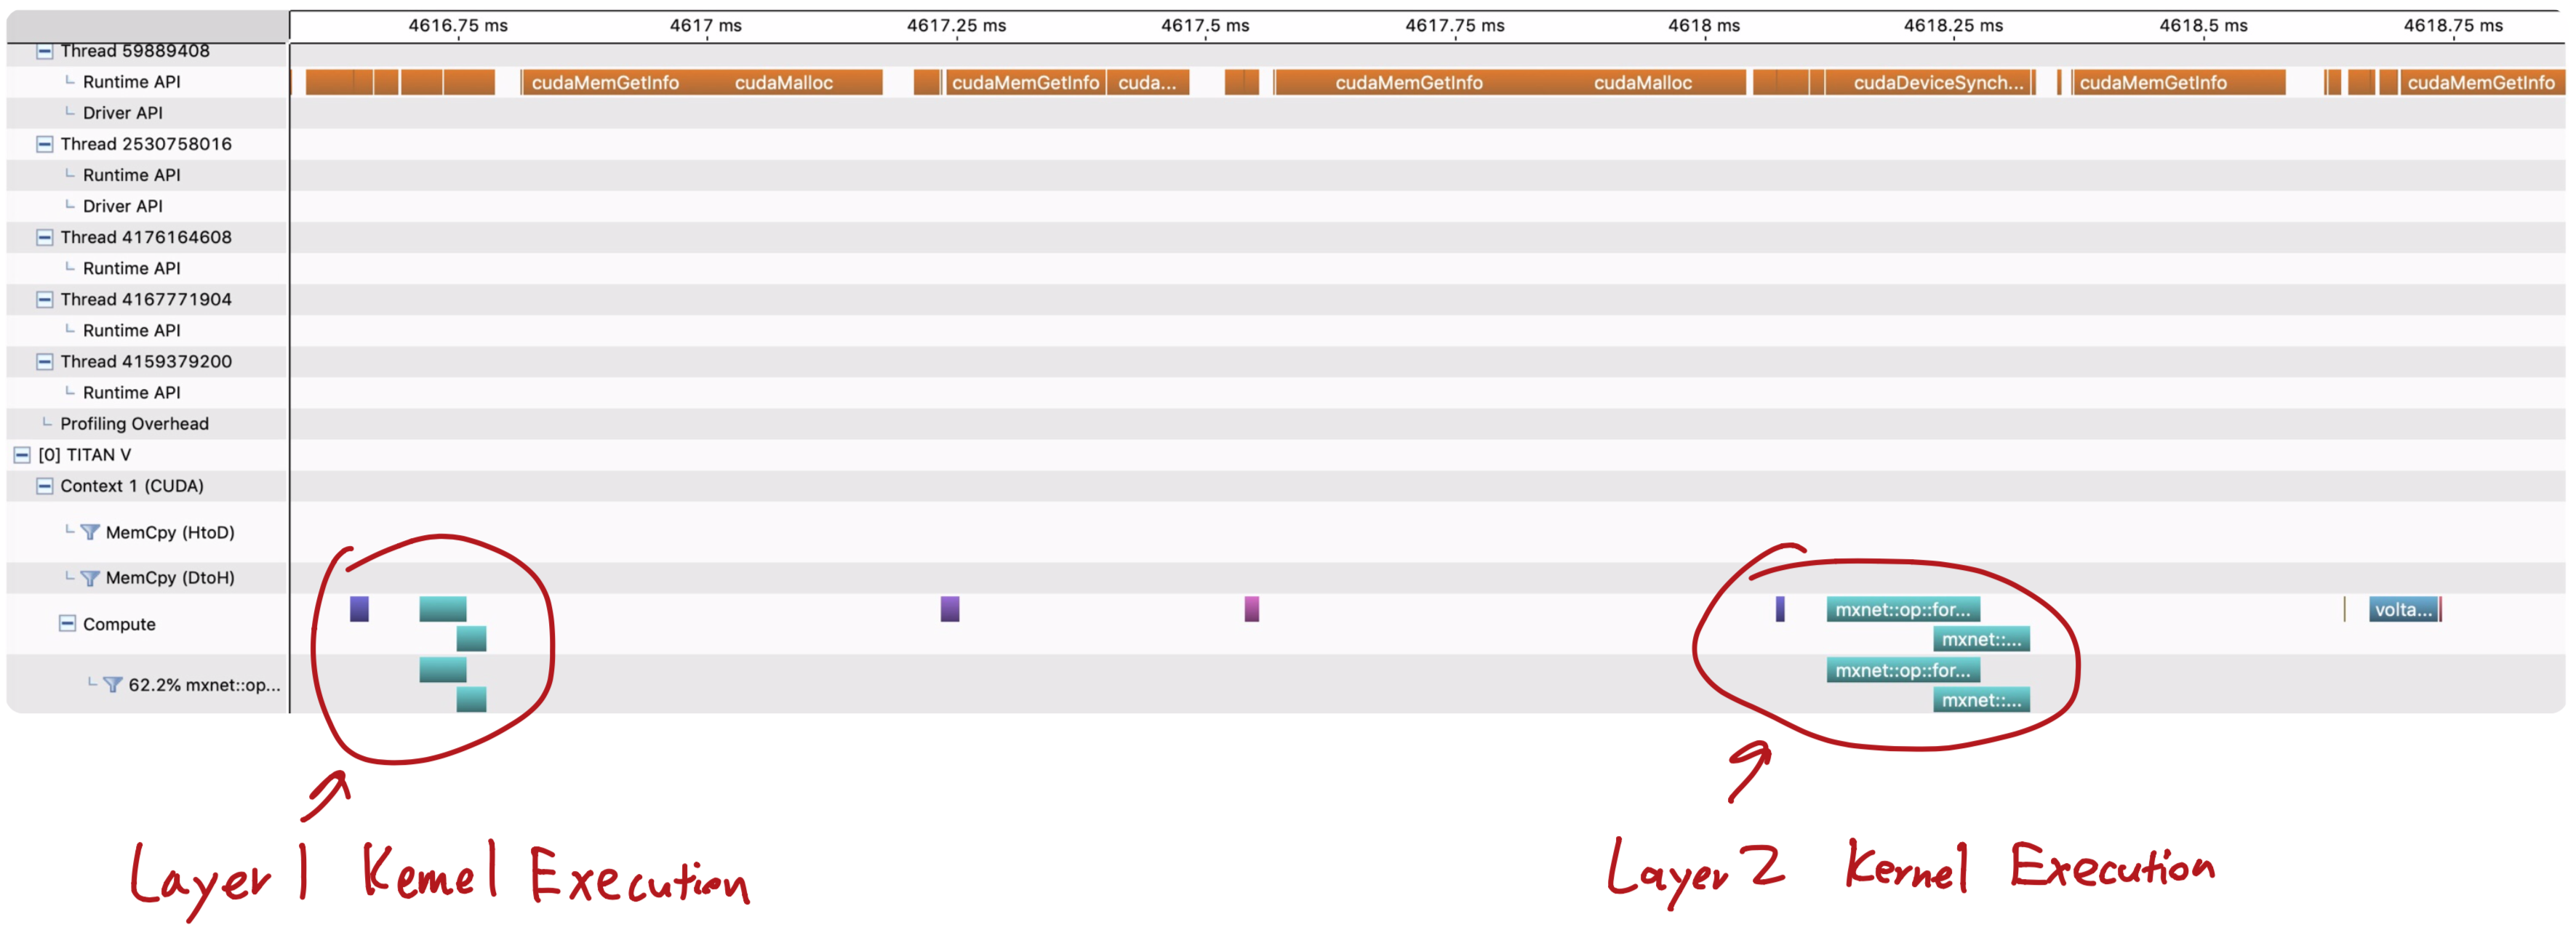
\includegraphics[width=\linewidth]{nvvp100an}
        \caption{Dataset Size 100}
    \end{subfigure}
    \begin{subfigure}[b]{\linewidth}
        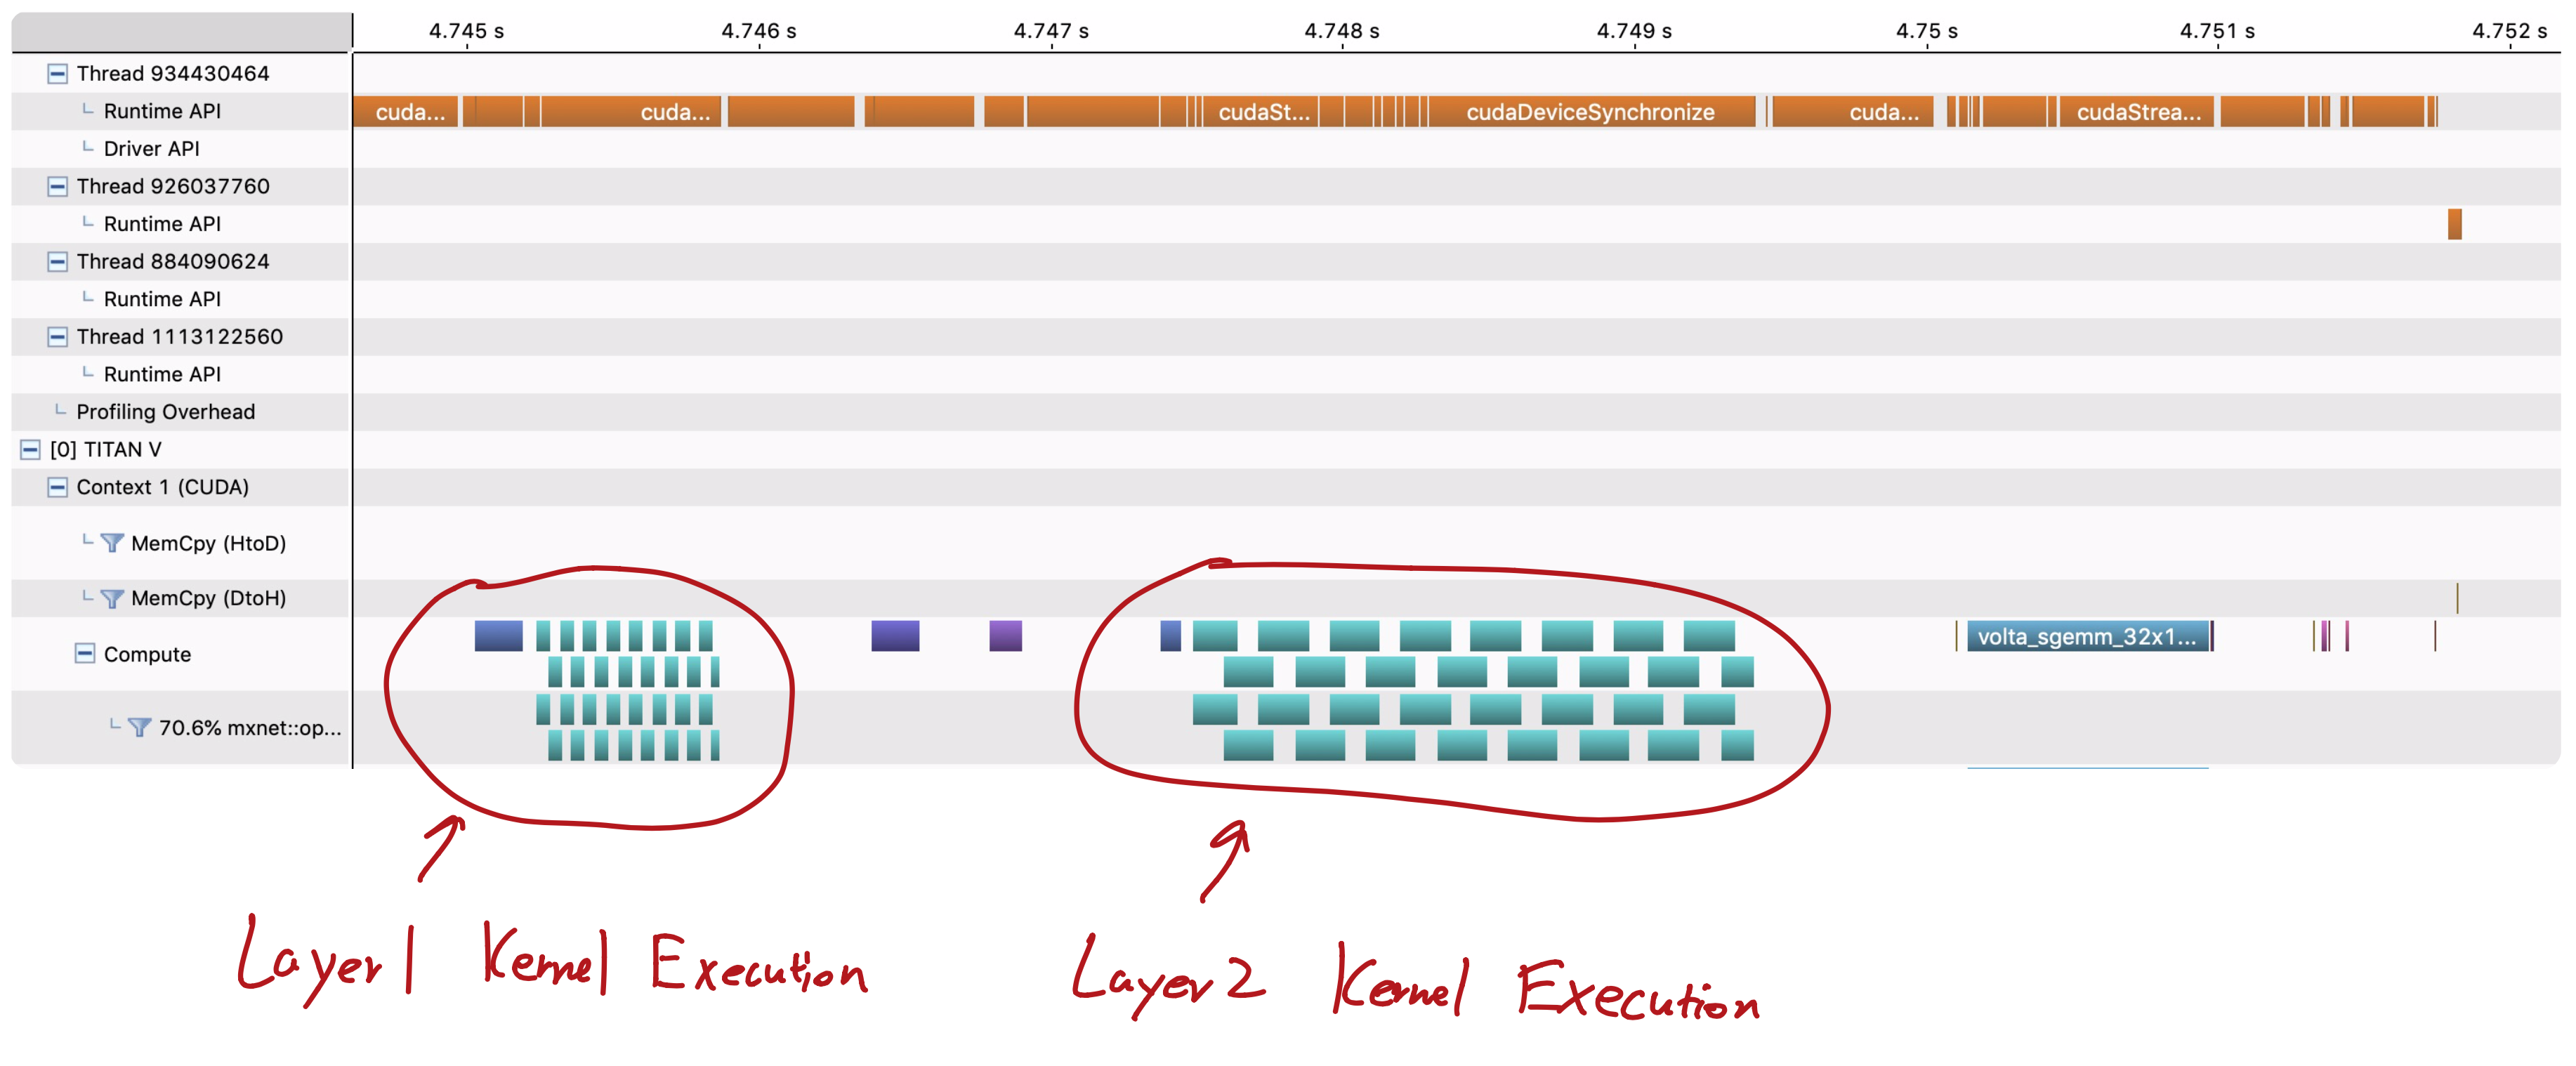
\includegraphics[width=\linewidth]{nvvp1000an}
        \caption{Dataset Size 1000}
    \end{subfigure}
    \begin{subfigure}[b]{\linewidth}
        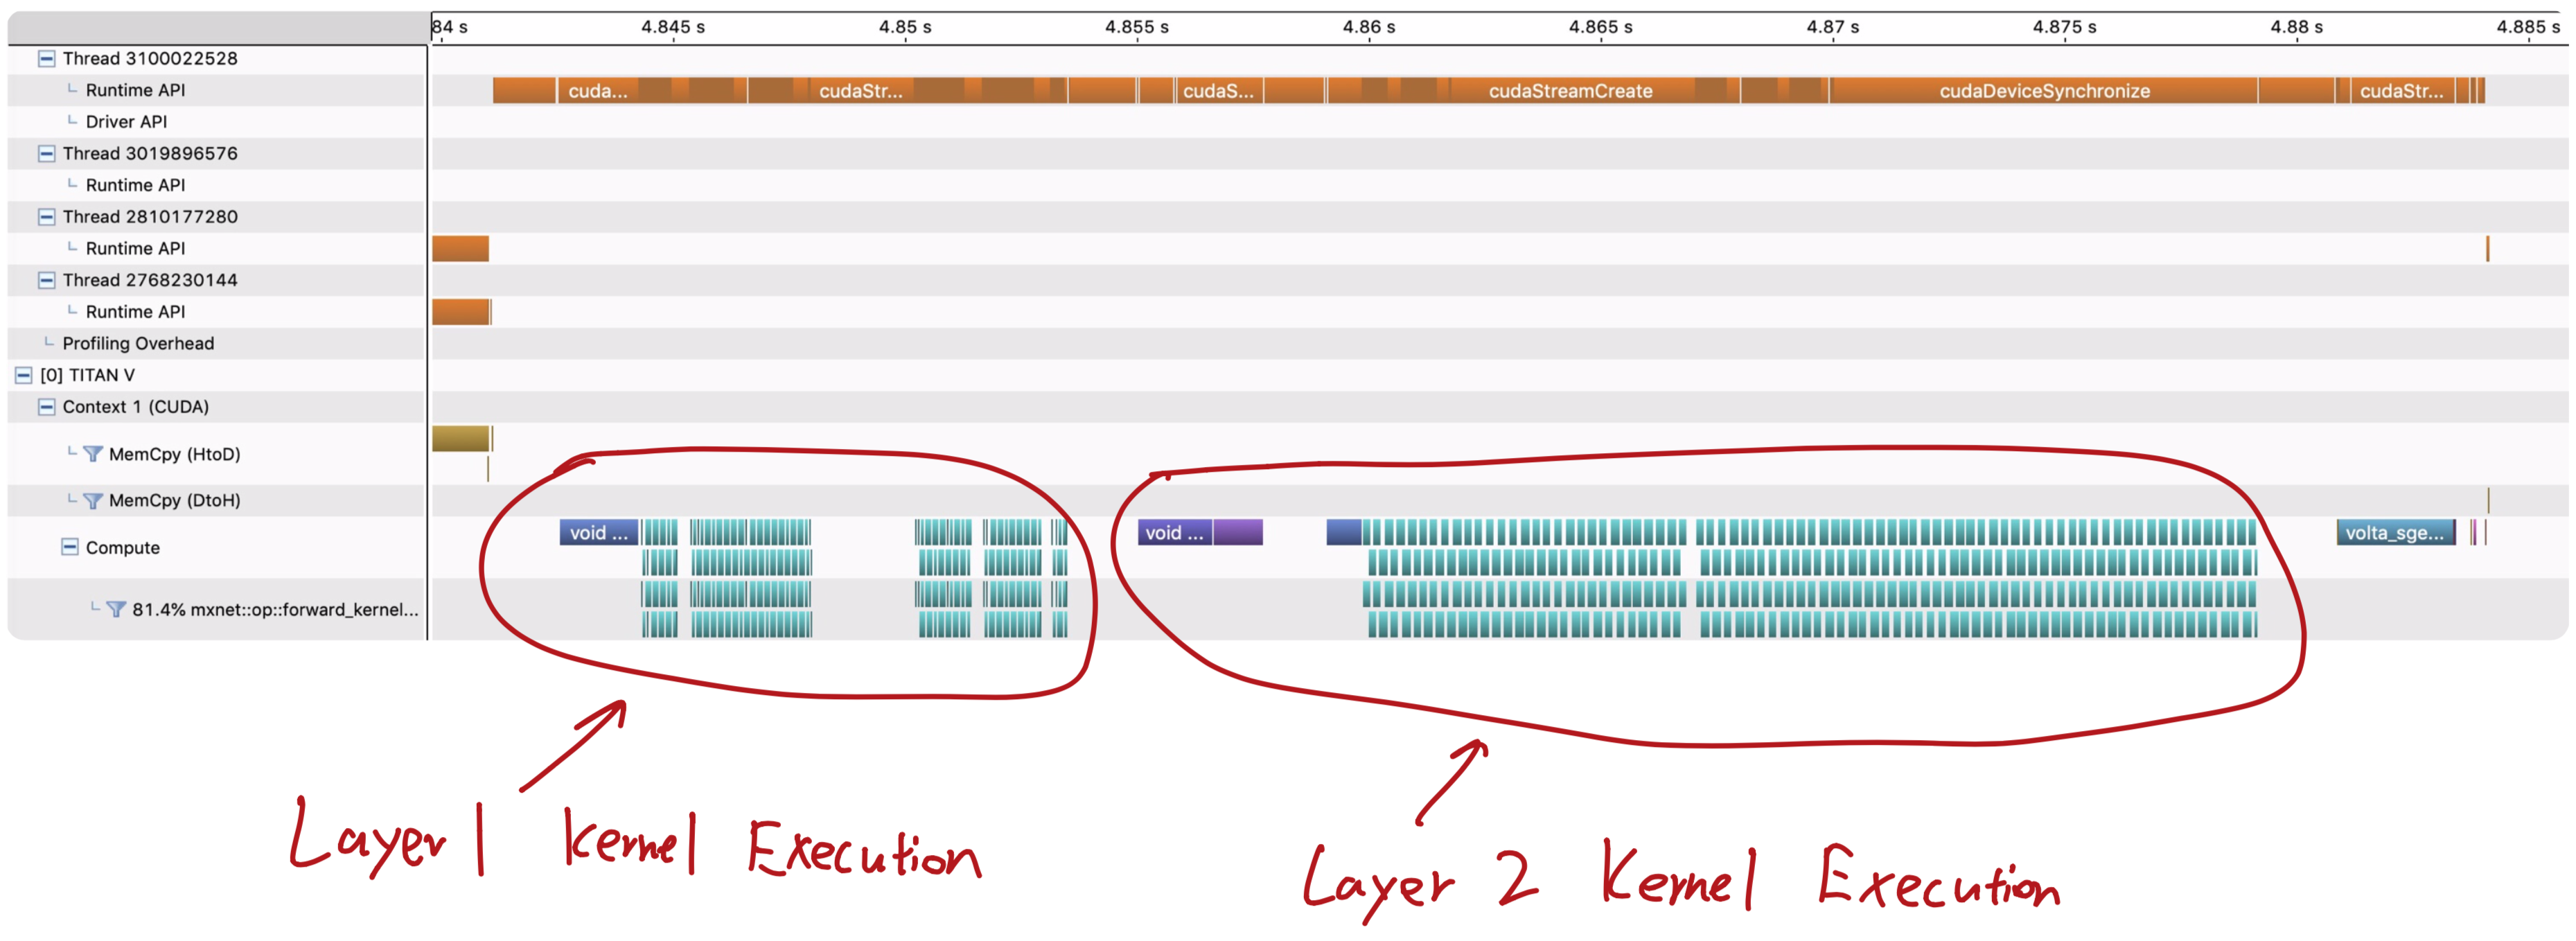
\includegraphics[width=\linewidth]{nvvp10000an}
        \caption{Datset Size 10000}
    \end{subfigure}
    \caption{Kernel Execution Timelines generated by NVVP.}
\end{figure}

\end{document}
